%%%%%%%%%%%%%%%%%%%%%%%%%%%%%%%%%%%%%%%%%%%%%%%%%%%%%%%%%%%%%%%%%%%%%%%%%%%%%%%%
% Author : [Sviatoslav] [Shishnev], Tomas Polasek (template)
% Description : Seventh exercise in the Introduction to Game Development course.
%   It deals with the creation of a Game Design Document, presenting a short 
%   pitch for a potential game project.
%%%%%%%%%%%%%%%%%%%%%%%%%%%%%%%%%%%%%%%%%%%%%%%%%%%%%%%%%%%%%%%%%%%%%%%%%%%%%%%%

\documentclass[a4paper,10pt,english]{article}

\usepackage[left=2.50cm,right=2.50cm,top=1.50cm,bottom=2.50cm]{geometry}
\usepackage[utf8]{inputenc}

% Hyper-Text References
\usepackage{hyperref}
\hypersetup{colorlinks=true, urlcolor=blue}

% Drawing Images and Graphs
\usepackage{tikz}
\usepackage{pgfplots}

% Page Utilities
\usepackage{graphicx}

% Image Sub-Captions
\usepackage{subcaption}

\newcommand{\ph}[1]{\textit{[#1]}}

\title{%
Game Pitch Document%
}
\author{%
Sviatoslav Shishnev (xshish02)%
}
\date{}

\begin{document}

\maketitle
\thispagestyle{empty}

{%
\large

\begin{itemize}

\item[] \textbf{Title:} Sacred spirits

\item[] \textbf{Genre:} JRPG or Japanese role play game

\item[] \textbf{Style:} 2D, Cartoon/Pixel style

\item[] \textbf{Platform:} PC, Consoles, Portable consoles

\item[] \textbf{Market:} 13/16/18+

\item[] \textbf{Elevator Pitch:} A young shaman, chosen for his spirit communication, embarks on a perilous continent-crossing ritual, navigating dense thickets, scaling towering peaks, and engaging in a ceremonial battle at a final gathering of fellow shamans.

\end{itemize}

}

\section*{\centering The Pitch}

\subsection*{Introduction}
The game is a 2D single-player role-playing adventure with platformer, puzzle, and adventure elements, as well as multiplayer components such as player-vs-player combat. The gameplay involves exploring new territories while following plot-related objectives. Players encounter challenges with multiple solutions based on their choices. Additionally, they must battle alongside spirit allies to overcome various dangers on their path to the ultimate goal.

\subsection*{Background}

The game's background draws inspiration from classic series like Megami Tensei, Pokemon, and Final Fantasy, which continue to thrive today. Our aim is not to replicate these series but to be inspired by their narrative and role-playing aspects. We aspire to tactical battles that captivate players with depth, in the spirit of the modern entries of Final Fantasy and Megami Tensei. We envision our game with a narrative resembling those series and the management of allied spirits similar to the recent Pokemon games. However, our goal is to introduce significant innovations in the tactical depth of the combat system to avoid player fatigue and attract new audiences.

\subsection*{Setting}
The events unfold on an island continent inhabited by people, animals, and spirits residing in suitable vessels. The society is divided into villages, representing city-states. Spirits are categorized as cursed (evil and cunning) and sacred (creative and benevolent). The island is in a dark age due to cursed spirits, disrupting trade, farming, and small settlements. The wild territories have become perilous, and only gifted shamans could face danger with less risk. The protagonist, one such shaman, embarks on a perilous and thrilling journey through abandoned lands. Encounters with survivors far from cities, adaptation alongside sacred spirits, and unraveling the mystery of the cursed spirits shape his path. The narrative includes multiple arcs, such as seeking the truth about cursed spirits, assembling a volunteer group to attack the cursed king—an antagonist who sent the spirits to the island. Non-linearity in the main questline offers various story endings based on decisions made in each arc.

\subsection*{Features}


\begin{itemize}
    \item \textbf{Unique Setting:} Set in a mysterious island continent with a diverse population of people, wild creatures, and spirits residing in vessels, creating a rich and immersive world.
    
    \item \textbf{Spiritual Connection:} The central theme of the game revolves around the protagonist's ability to communicate and form bonds with spirits, offering a unique gameplay element.
    
    \item \textbf{Dual Nature of Spirits:} The division of spirits into cursed and sacred, each with distinct characteristics, adds depth to the narrative and strategic choices for players.
    
    \item \textbf{Dark Age Challenge:} The narrative backdrop of a dark age, caused by the invasion of cursed spirits, provides a compelling challenge for players to overcome and rebuild.
    
    \item \textbf{Nonlinear Storytelling:} The inclusion of multiple story arcs with branching paths and different endings based on player decisions adds replay value and encourages diverse playstyles.
    
    \item \textbf{Tactical Depth in Combat:} The promise of innovative tactical depth during battles, departing from the conventional gameplay found in similar genres, provides a fresh and engaging experience for players.
    
    \item \textbf{Character Growth and Discovery:} Players accompany the protagonist on a journey of self-discovery and growth as a shaman, learning about the intricacies of spirits and their development.
    
    \item \textbf{Mystery and Exploration:} The game emphasizes exploration of abandoned lands, unraveling the mystery behind cursed spirits, and discovering the untold stories of survivors, adding an element of intrigue.
    
    \item \textbf{Strategic Group Building:} Assembling a group of volunteers for a final showdown against the cursed king provides strategic depth, encouraging players to think tactically and make impactful choices.
    
    \item \textbf{Dynamic Dark Fantasy Style:} The game adopts a dark fantasy style, offering a casual experience but transitioning to brighter tones in safe places to evoke a sense of safety for players. This stylistic choice aligns with the popularity of dark fantasy, as seen in projects like Elden Ring, Souls series, and The Witcher, enhancing the game's appeal to fans of the genre, which are going crazy these days.
\end{itemize}

\subsection*{Genre}
\textbf{Dark Fantasy Tactical Role-Playing Game (TRPG)}

\subsection*{Nuances that Set it Apart:}

\begin{itemize}
    \item \textbf{Spiritual Emphasis:} Diverging from traditional JRPGs, our TRPG places a strong emphasis on the protagonist's spiritual connection with a diverse range of spirits, introducing unique gameplay mechanics and strategic choices reminiscent of the Pokemon series.
  
    \item \textbf{Tactical Depth in Combat:} Inspired by the strategic elements found in tactical RPGs, our game introduces innovative combat mechanics, offering a fresh experience for players accustomed to both JRPG and TRPG genres.
  
    \item \textbf{Dynamic Stylistic Shifts:} The game features a dynamic dark fantasy style, seamlessly transitioning between a dark and foreboding atmosphere to brighter tones in safe havens. This stylistic choice enhances the player's emotional engagement and provides a unique touch within the JRPG/TRPG genre.
  
    \item \textbf{Nonlinear Storytelling:} Our game offers multiple story arcs with branching paths and different endings, providing players with a more personalized and replayable experience.
\end{itemize}

\subsection*{Platform}
The initial release is strategically planned for PC (Windows), Nintendo Switch, and the recently introduced Steam Deck, aligning with the portable nature of these consoles that complements our game genre. Following a successful launch and based on player demand, we plan to expand to other PC platforms such as Linux and macOS. Additionally, we aim to make the game accessible to a broader console audience by releasing versions for PlayStation and Xbox. As the game gains traction and popularity, there's potential for adaptation to mobile platforms like iOS and Android, ensuring a versatile availability across a spectrum of gaming devices.

\subsection*{Style}
\emph{The Game} immerses players in a visually stunning realm where the tranquility of Eastern themes converges with the mystique of dark fantasy, forging a unique and captivating aesthetic.

\begin{itemize}
    \item \textbf{Eastern-Inspired Architecture:} Envision villages and cities adorned with intricately crafted wooden structures, pagodas, and torii gates. The architectural design draws inspiration from various cultures of the East, infusing the game world with a rich cultural tapestry.
  
    \item \textbf{Tactical Combat Visuals:} Engage in battles amidst lush bamboo forests and serene cherry blossom groves. Tactical moves and spirit interactions are brought to life with fluid animations that reflect the elegance and precision of Eastern martial arts.
  
    \item \textbf{Harmonious Contrasts:} Safe zones emanate a sense of peace and harmony. Wooden bridges span over gentle streams, lantern-lit paths wind through tranquil gardens, and cherry blossoms gently fall, creating serene visuals that offer respite from the darker aspects of the game.
  
    \item \textbf{Character Design and Growth:} Characters evolve with a nod to Eastern aesthetics, reflecting the journey from apprentice to seasoned shaman. Traditional garments, adorned with symbolic elements, mirror the character's growth and connection with the spirits.
  
    \item \textbf{Environmental Storytelling:} Explore landscapes infused with Eastern symbolism. Ancient shrines, bamboo groves, and mystical waterfalls narrate tales of spirits, adding depth to the overall narrative through the visual language of the environment.
\end{itemize}

In summary, picture a world where the elegance of Eastern aesthetics meets the intrigue of dark fantasy, inviting players to embark on a visually enchanting journey in \emph{Sacred spirits game}.

\begin{figure}[h]
\centering

\begin{subfigure}{0.70\linewidth}
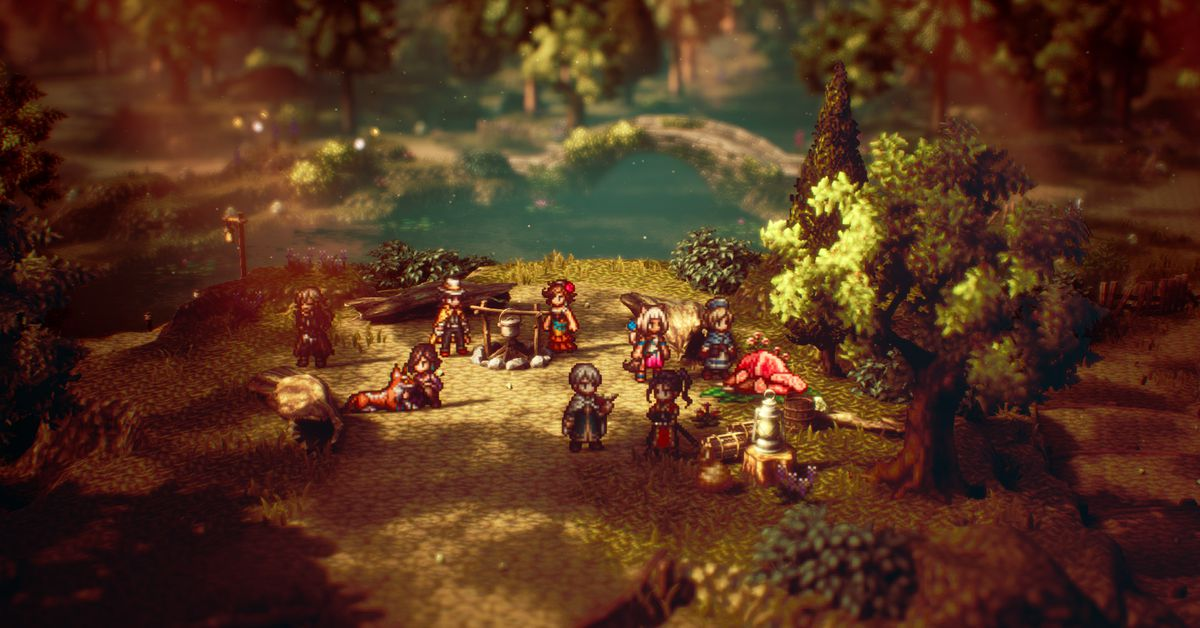
\includegraphics[width=\linewidth]{style1.jpg}
\captionof{figure}{Inspiration from Octopath traveller}
\label{Fig:Style1A}
\end{subfigure}\hfill
%
\begin{subfigure}{0.70\linewidth}
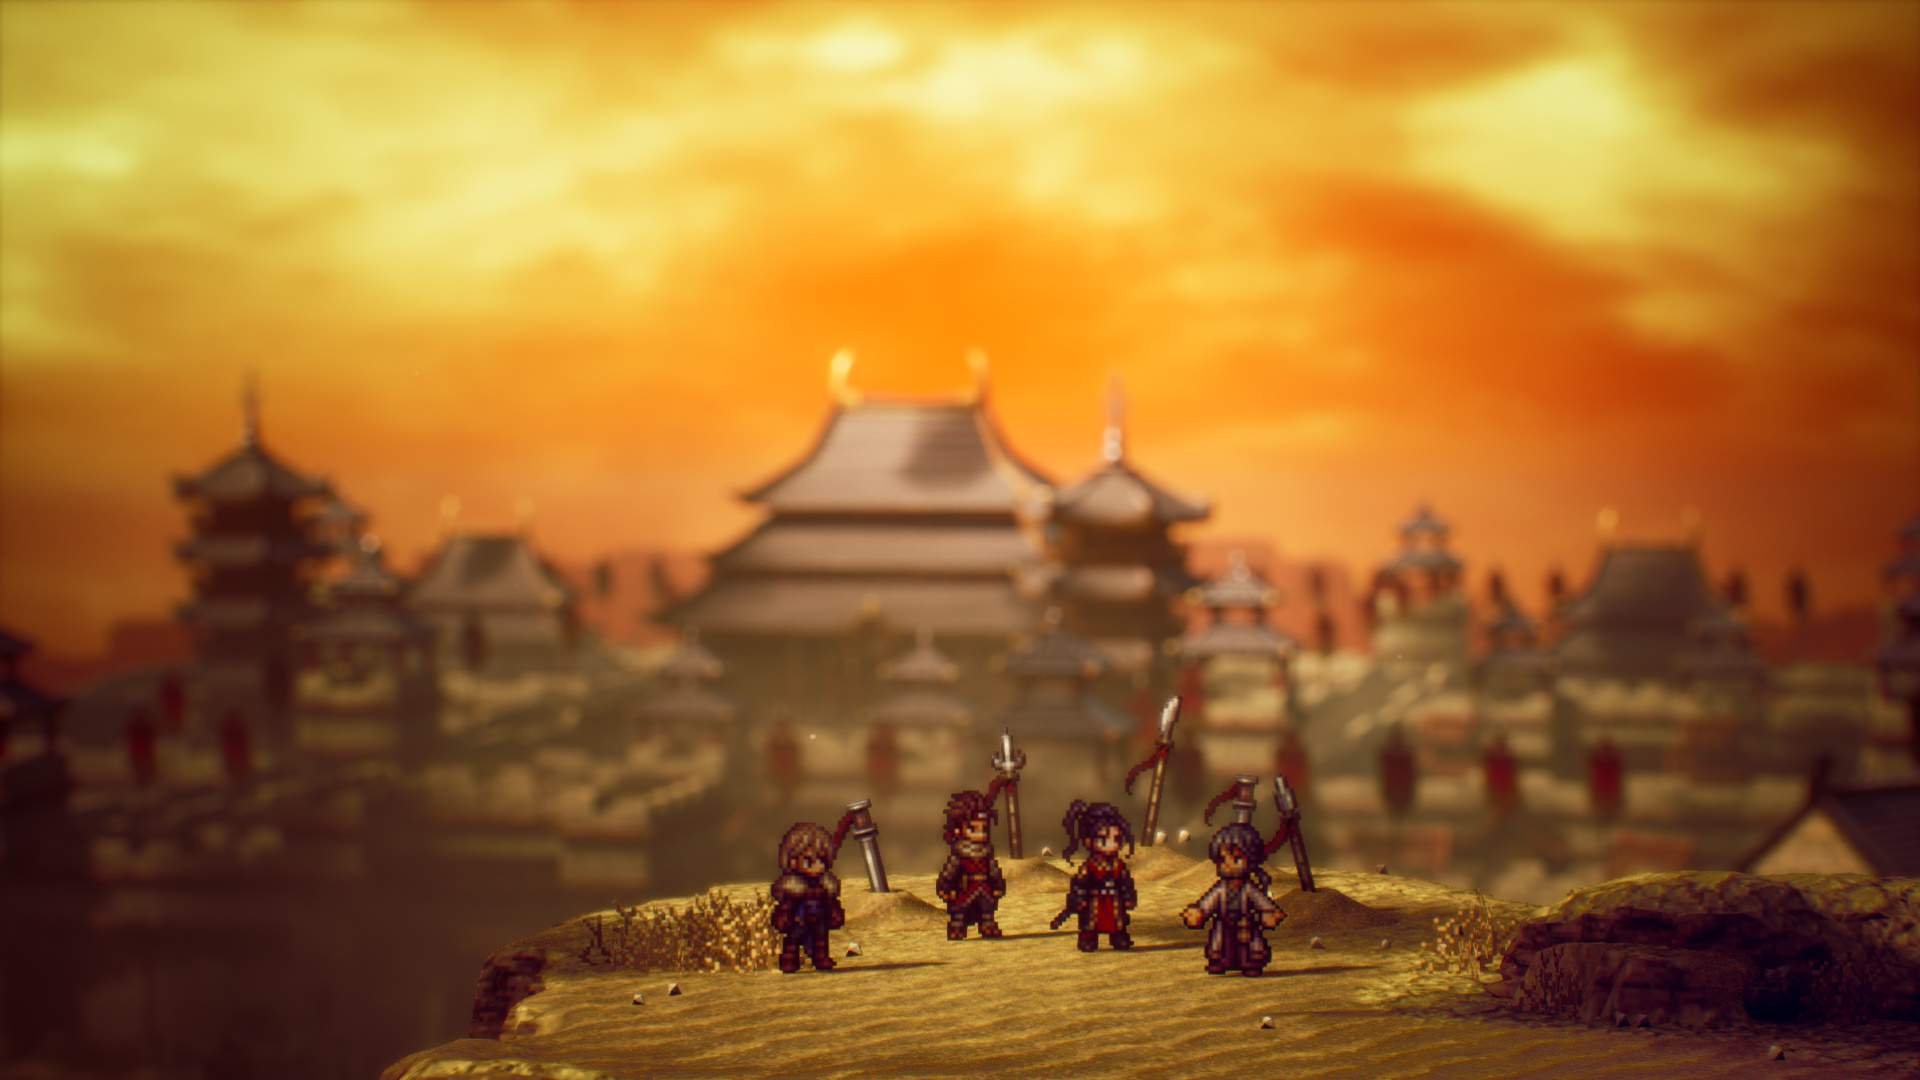
\includegraphics[width=\linewidth]{style2.jpg}
\captionof{figure}{Inspiration from Octopath traveller}
\label{Fig:Style1B}
\end{subfigure}\hfill
%


\begin{subfigure}{0.70\linewidth}
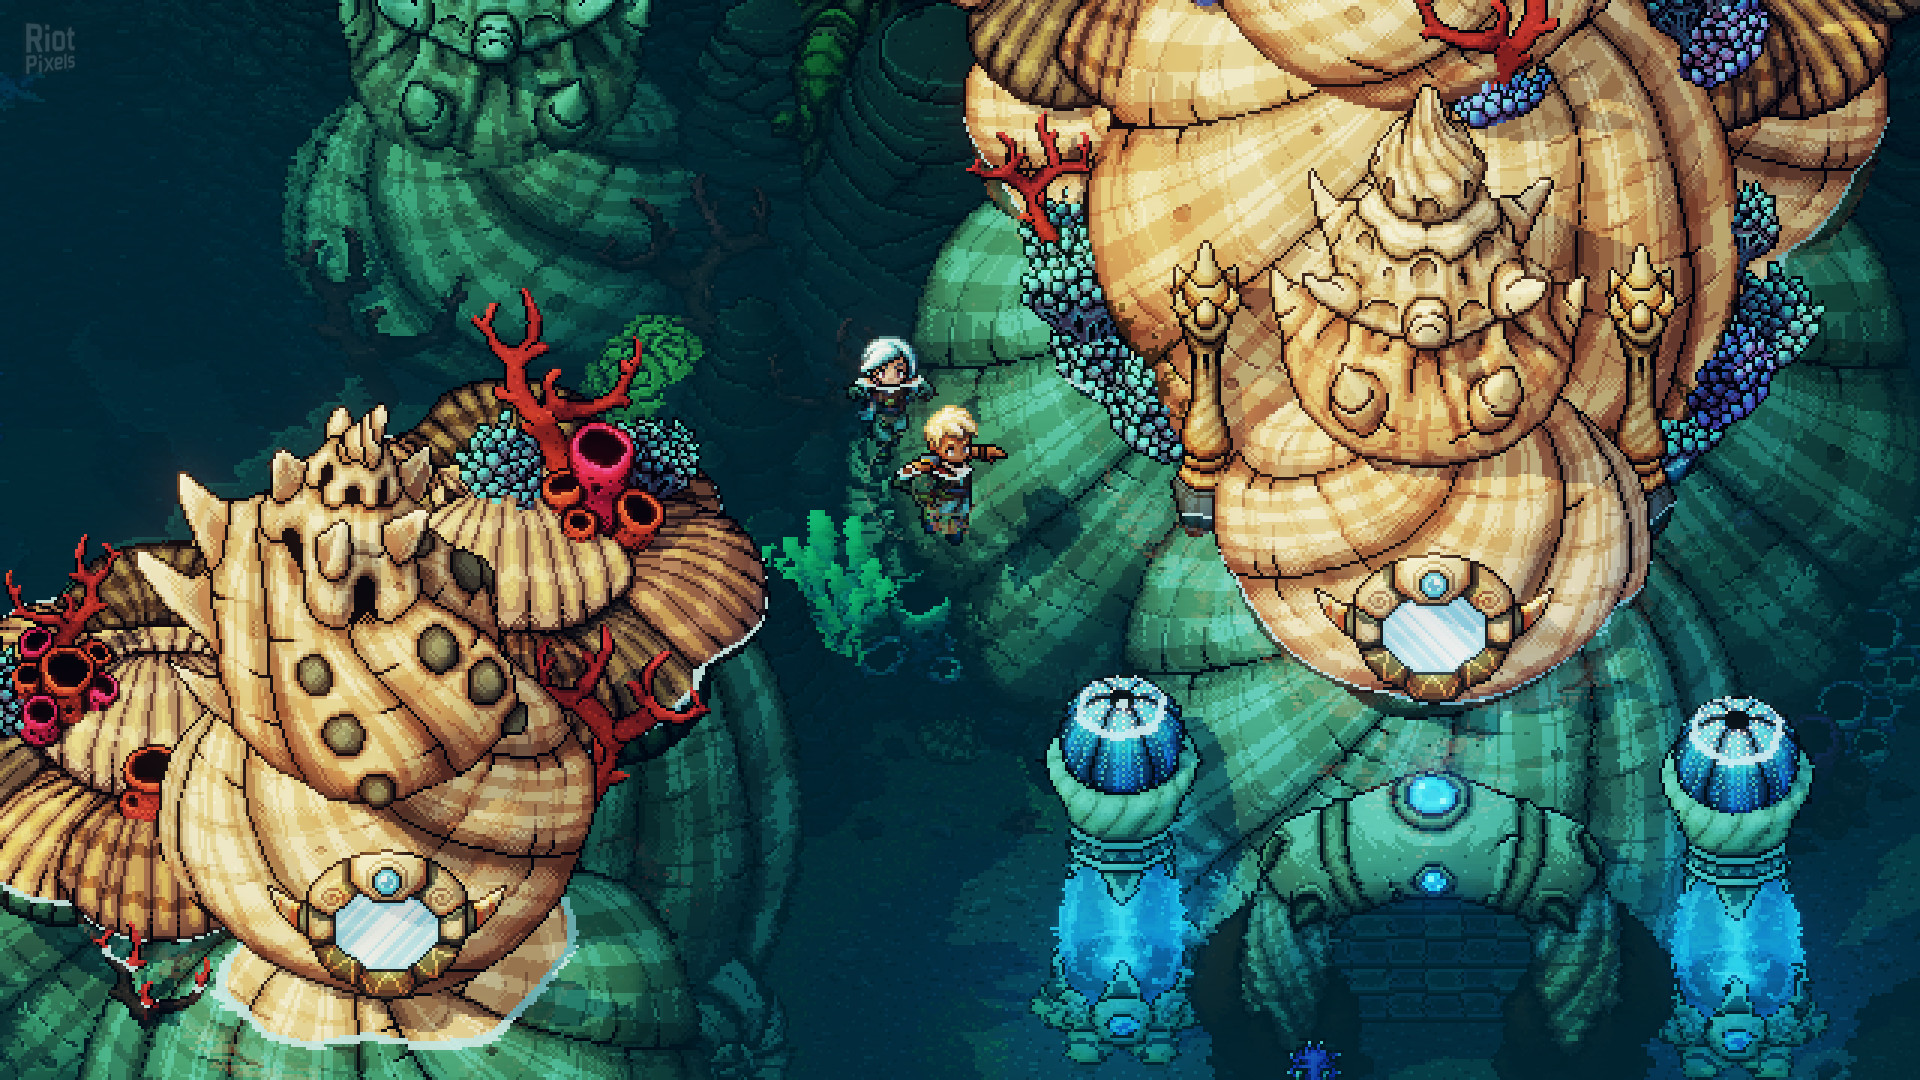
\includegraphics[width=\linewidth]{style5.jpg}
\captionof{figure}{Inspiration from Sea of stars}
\label{Fig:Style1C}
\end{subfigure}


\end{figure}


\end{document}
